% Document
% Document
\documentclass[12pt, a4paper]{article}
\usepackage[T1]{fontenc}
\usepackage[utf8]{inputenc}
\usepackage{authblk}
\usepackage{lipsum}
\usepackage{tikz}
\usepackage{hyperref}

% Figure and table formating
\usepackage{epsfig}
\usepackage{tabu}
\usepackage{rotating}
\usepackage{pbox}
\usepackage{framed, multicol}
\usepackage[framemethod=TikZ]{mdframed}

% Set up Frame
\mdfdefinestyle{MyFrame}{%
    linecolor=black,
    skipabove=10pt,
    outerlinewidth=2pt,
    roundcorner=20pt,
    innertopmargin=10pt,
    innerbottommargin=10pt,%\baselineskip,
    innerrightmargin=20pt,
    innerleftmargin=20pt,
    backgroundcolor=gray!50!white}

\usepackage{float}
\usepackage[left=1 in, right=1 in, top=1.25 in, bottom=1.25 in]{geometry}

% Fonts - Mathtime
%\usepackage{txfonts}
\usepackage{amsmath} % Add amssymb if not using Mathtime

% Text
\setlength{\parindent}{0.5in}
\frenchspacing  \tolerance = 800  \hyphenpenalty = 800

\usepackage{lineno} % Line numbers
\def\linenumberfont{\normalfont\footnotesize\ttfamily}
\setlength\linenumbersep{0.1 in}

\usepackage{setspace}

% Other
\usepackage{graphicx}
\usepackage[singlelinecheck=false,font=small,labelfont=bf]{caption}

\begin{document}
\thispagestyle{empty}

\begin{figure}

\begin{tikzpicture}


    \node at (0, 0) (pic) {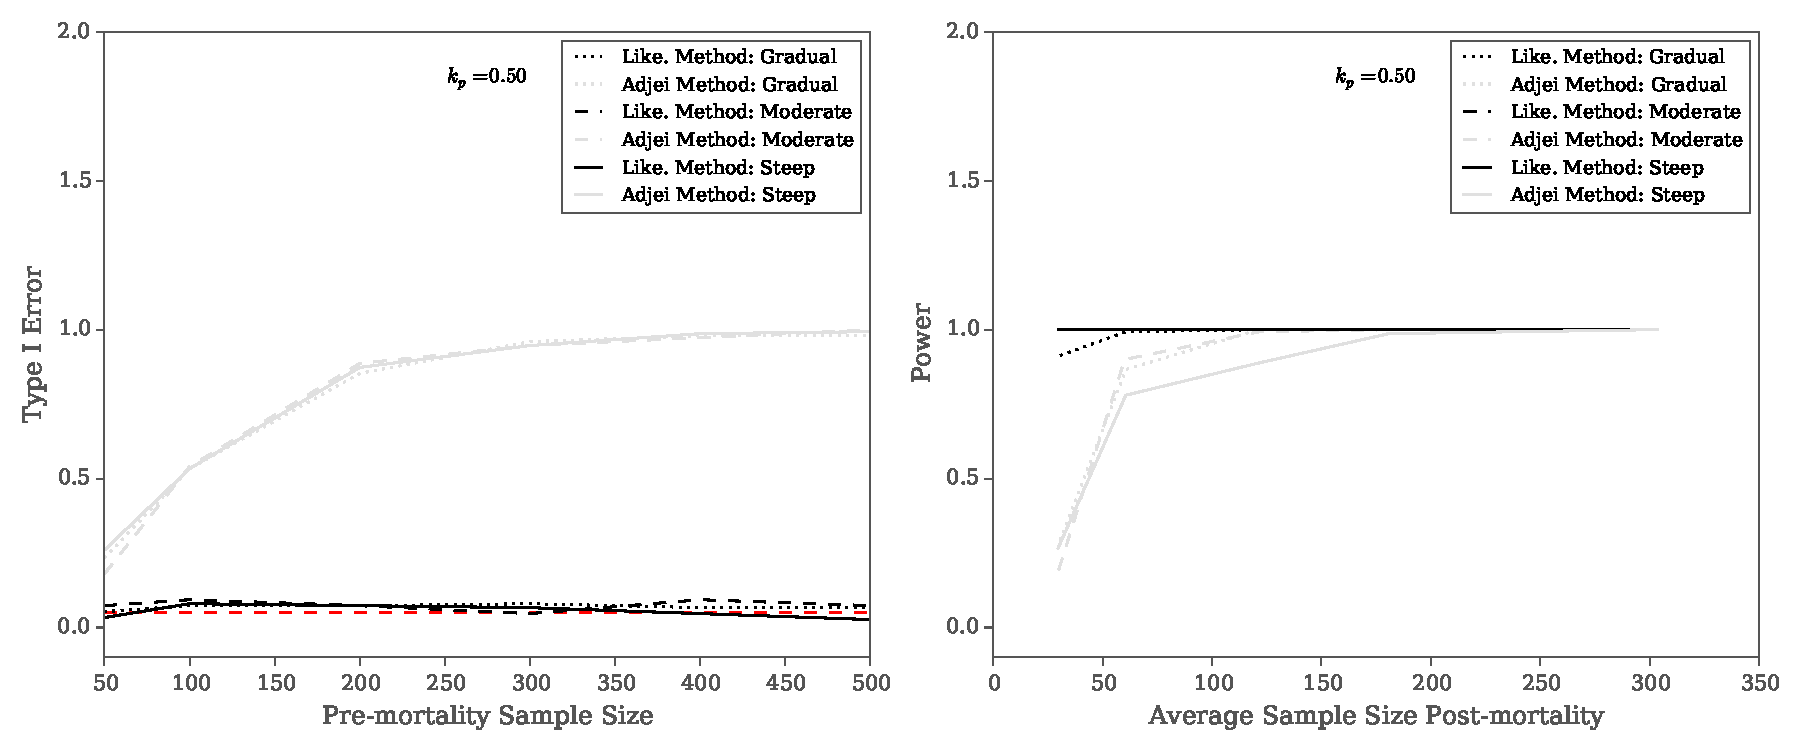
\includegraphics[width=\textwidth]{/Users/mqwilber/Repos/parasite_mortality/results/figure1_partII_for_manuscript50}};

    \node[above=0.1cm] at (pic.north) (concept) {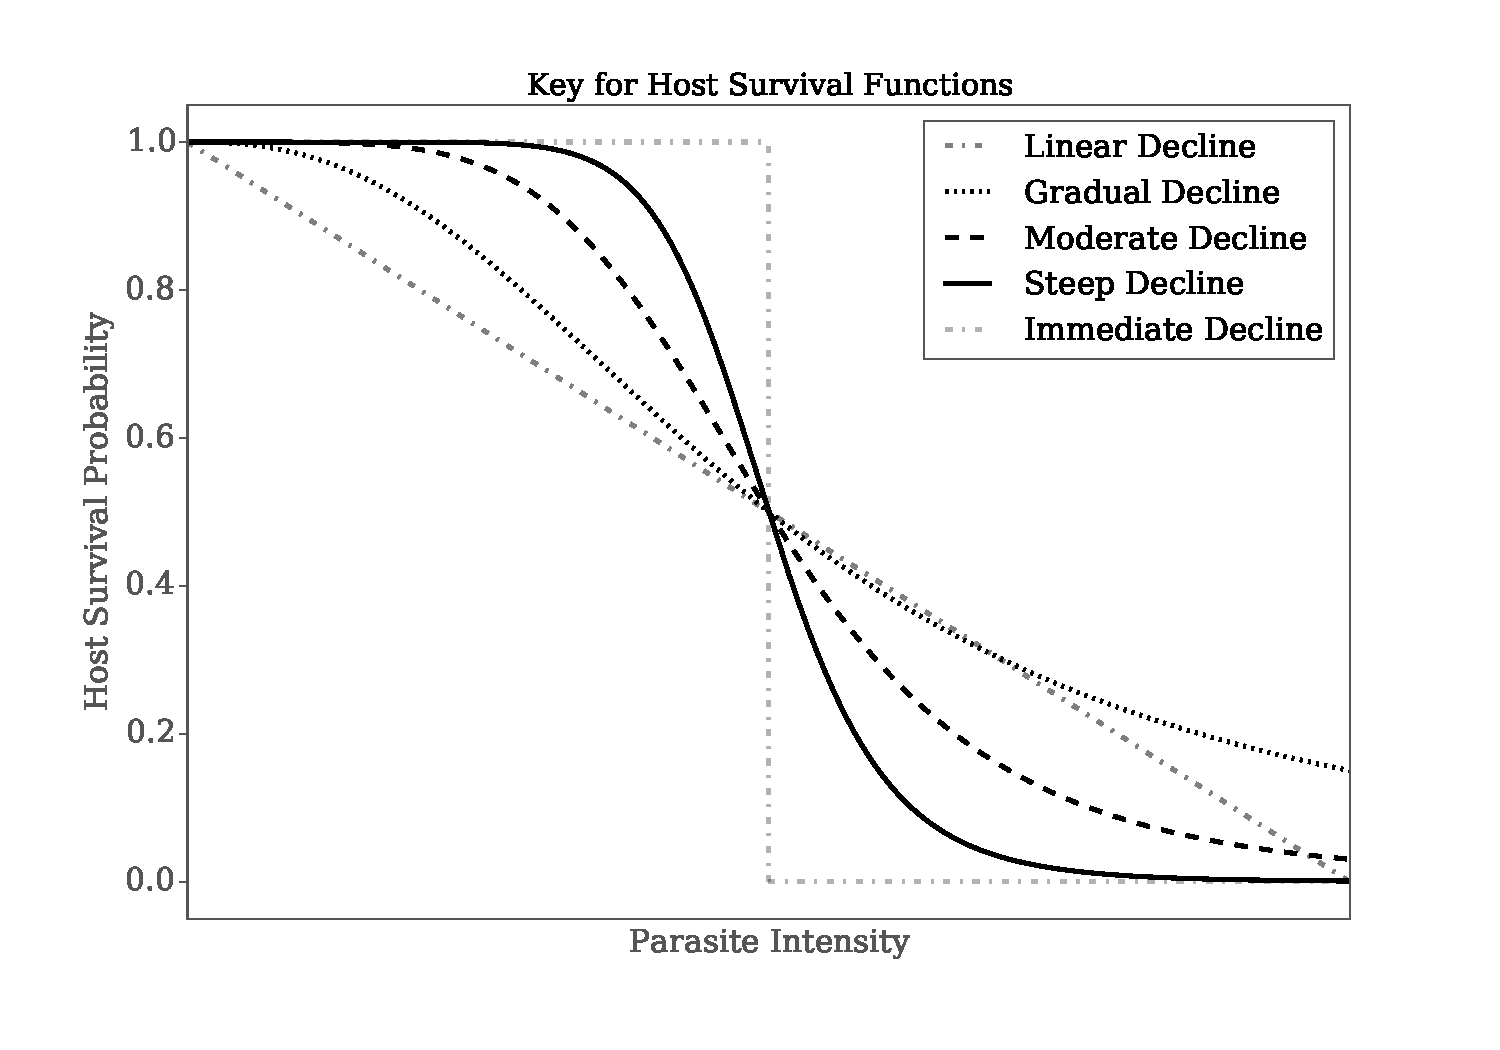
\includegraphics[width=0.6\textwidth]{/Users/mqwilber/Repos/parasite_mortality/results/figure1_partI_for_manuscript}};

    \draw[->] (0, 4.2)--(-1.5, 3.2);
    \draw[->] (0, 4.2)--(1.5, 3.2);

    \node at (-3.2, 4.9) {A.};
    \node at (-6.7, 2.9) {B.};
    \node at (1.15, 2.9) {C.};

\end{tikzpicture}

\end{figure}

\centering

\textbf{Figure 2}

\end{document}